% Use 8.5 x 11 standard A4 paper for printing optimization in US
\documentclass[a4paper]{article}
\usepackage{float}
\marginparsep = 0pt
\marginparwidth = 0pt
\textwidth=6.0in
\oddsidemargin = 0.0in
\evensidemargin = 0.0in
\usepackage{graphicx}
\usepackage{hyperref}
\linespread{1.1}% spread lines out a little
\newcommand{\yobs}{y_{obs}}
\newcommand{\yatm}{y_{atm}}
\setcounter{tocdepth}{5}
\begin{document}

\begin{center}
\bf \large Airmass Calculator
\end{center}

This calculator was designed to calculate the airmass $X$ that an observer at non-zero elevations $\yobs$ (height above sea-level) would measure for objects at various altitudes $\alpha$ (angular heights above the horizon) compared to an observer at sea-level. By definition, the airmass for a target at the zenith is unity at sea-level, and we define relative airmass such that $X < 1$ for targets at the zenith at elevations $\yobs > 0$. 

{\bf Some definitions:} We define the zenith angle $z = \pi/2 - \alpha$, the radius of the earth $R_e = 6371$ km, the height above sea-level of the observer $\yobs$, the height above sea-level where the atmosphere becomes negligible $\yatm = 100$ km (the ``Karman line''), the atmospheric density $\rho$ which is a function of elevation,  the column density $\sigma$ and the path length of light through the atmosphere to the observer $s$. 

\begin{figure}[H]
\begin{center}
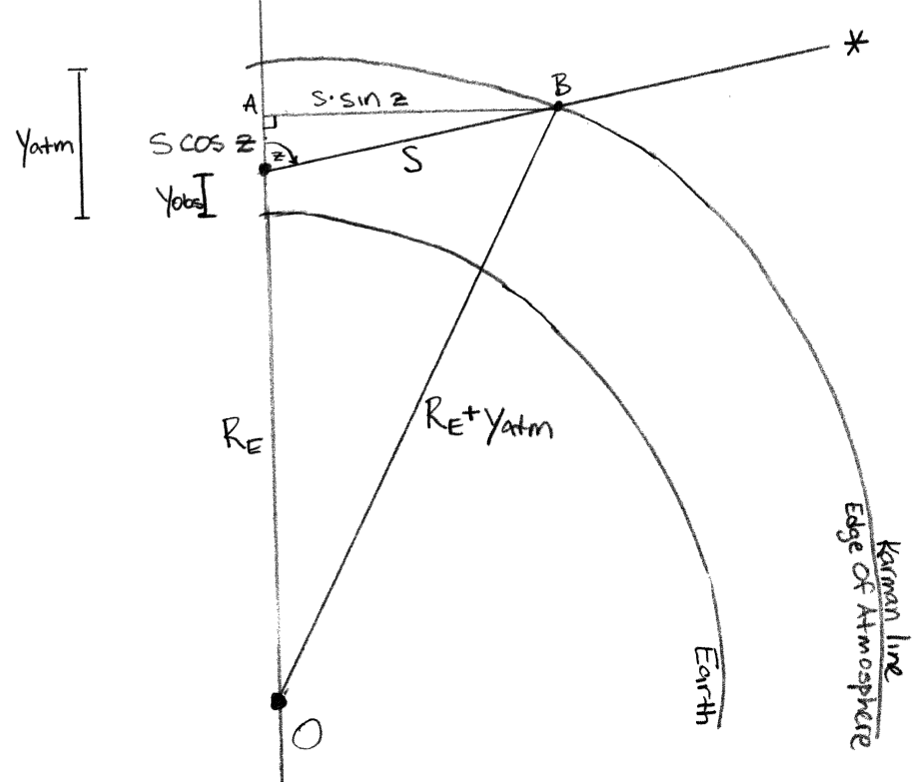
\includegraphics[scale=0.34]{figs/diagram.png}
\caption{Geometric defintions}
\end{center}
\end{figure}

From triangle OAB, we see that 
\begin{equation}
(R_e + \yobs + s \cos z )^2 + (s \sin z)^2 = (R_e + \yatm)^2
\end{equation}
Manipulating this relation we can find the quadratic in $s$
\begin{equation}
s^2 + 2 \cos z (R_e + \yobs) s + \yobs^2 - \yatm^2 + 2R_e(\yobs-\yatm) = 0.
\end{equation}
The roots are 
\begin{equation}
s = \pm \sqrt{ (R_e + \yobs)^2\cos^2 z - \yobs^2 + \yatm^2 - 2R_e(\yobs-\yatm)} - (R_e + \yobs)\cos z \label{eqn:s}, 
\end{equation}
and we take only the positive solution since we are solving for a positive path length $s$. 

The column density of atmosphere along the path $s$ for an atmosphere of variable density $\rho$ is 
\begin{equation}
\sigma = \int \rho ~ ds. \label{eqn:sig}
\end{equation}
Notice that in Eqn.~\ref{eqn:s} we have found $s=s(\yatm)$, we can say more generally that the path length to a given height in the atmosphere $y$ is 
\begin{equation}
s(y) = \sqrt{ (R_e + \yobs)^2\cos^2 z - \yobs^2 + y^2 - 2R_e(\yobs-y)} - (R_e + \yobs)\cos z,
\end{equation}
and we can change variables in Eqn.~\ref{eqn:sig} to exchange $s$ for height in the atmosphere $y$, using $ds = \frac{ds}{dy} dy$, 
\begin{eqnarray}
\frac{ds}{dy} &=& \frac{R_e + y}{\sqrt{ (R_e + \yobs)^2\cos^2 z - \yobs^2 + y^2 - 2R_e(\yobs - y) }},\\
\sigma(\yobs,z) &=& \int^{\yatm}_{\yobs}  \frac{\rho(y)~\left(R_e + y\right)~dy}{\sqrt{ (R_e + \yobs)^2\cos^2 z - \yobs^2 + y^2 - 2R_e(\yobs - y) }}
\end{eqnarray}
The density of the atmosphere as a function of height $\rho(y)$ is interpolated from the US Standard Atmosphere (1976 version). 


The relative airmass $X$ given by the calculator for a target at zenith angle $z_0$, for an observer at elevation $y_0$ is
\begin{equation}
X = \frac{\sigma(\yobs=y_0,z=z_0)}{\sigma(\yobs=0,z=0)}.
\end{equation}


Below we compare this definition of $X$ (labelled ``Morris'') to the simple $X \approx \sec z$ approximation often used, as in the package ``SkyCalc'':
\begin{figure}[H]
\begin{center}
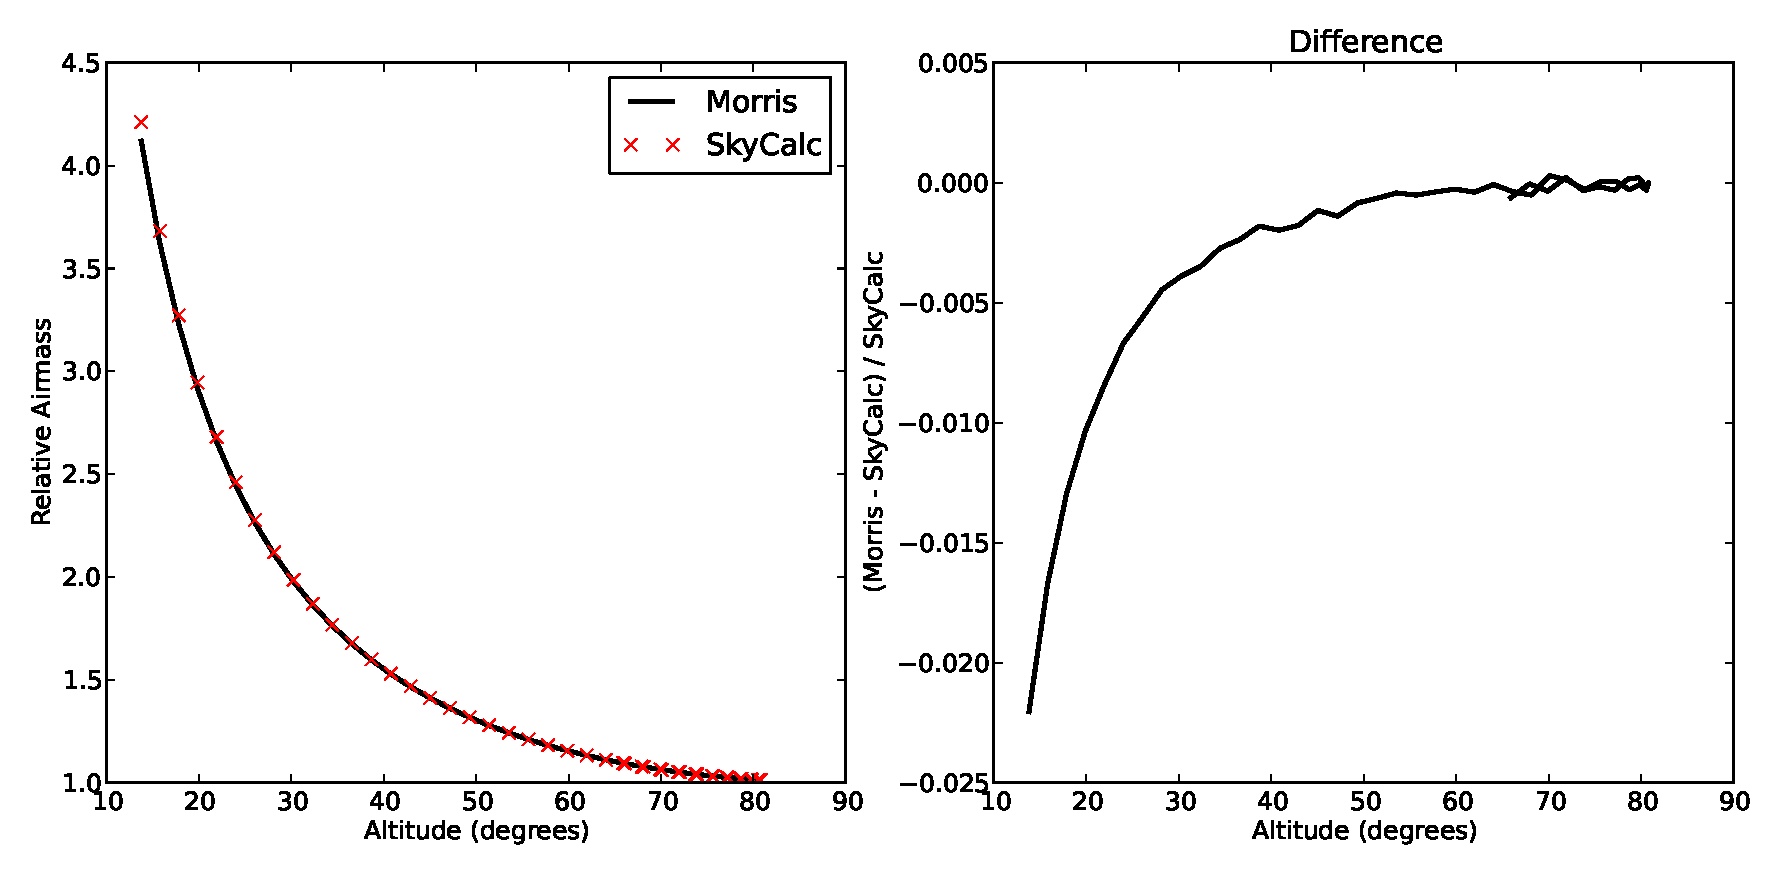
\includegraphics[scale=0.5]{figs/validation.eps}
\caption{Validation by comparison to the common approximation $X \approx \sec z$.}
\end{center}
\end{figure}

\end{document}